\begin{wrapfigure}[28]{r}[0pt]{115mm}
%	\centering
    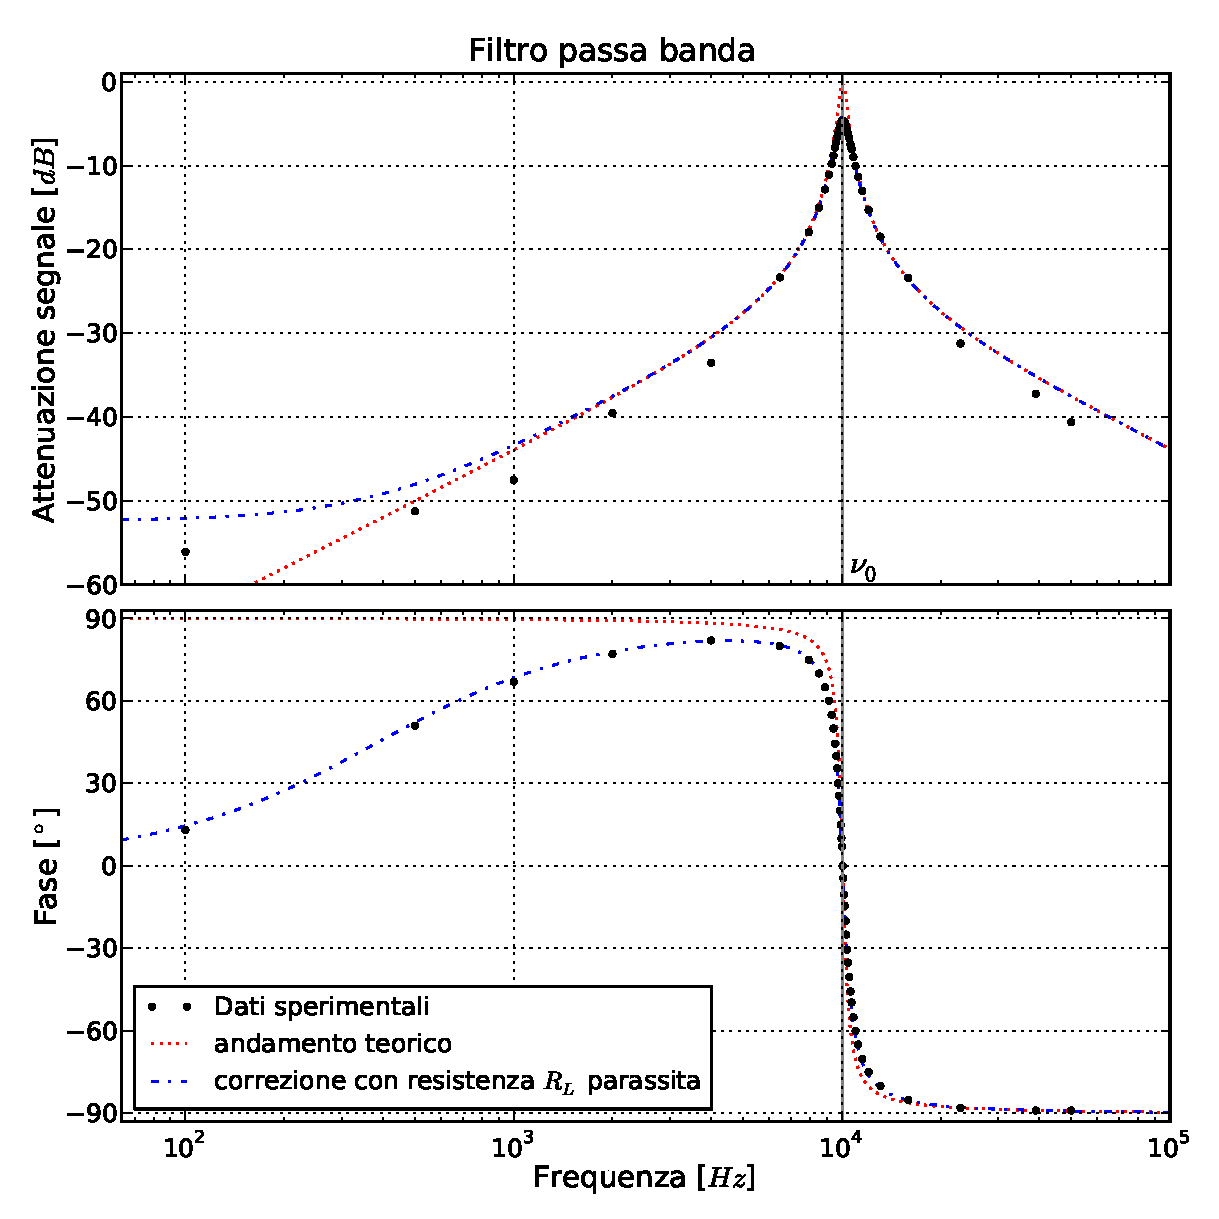
\includegraphics[width=120mm]{bpf.pdf}
    \caption{Diagrammi di Bode per il filtro passa banda.}
    \label{fig:bpf}
\end{wrapfigure}

\section{Passa banda}
Questo secondo filtro analizzato, oltre che resistenza e condensatore, prevede l'utilizzo di un'induttanza. In Fig. \ref{fig:circuito} è rappresentato il circuito utilizzato. Il parallelo di induttanza e condensatore fa sì che sia per frequenze basse che per quelle alte l'oscilloscopio sia cortocircuitato. Infatti l'induttanza si comporta come filo ideale per frequenze basse mentre come circuito aperto per quelle alte. Tale filtro lascerà passare dunque solo un range di frequenze attorno al valore $\nu_0$, detta frequenza di risonanza e definita come $\nu_0=\frac{1}{2 \pi \sqrt{LC}}$. Per questo motivo abbiamo deciso di prendere misure circa ogni $5^\circ$ a salire e a scendere in frequenza partendo da $\nu_0$.

Come fatto nel paragrafo precedente, è possibile utilizzare il concetto di partitore generalizzato per risolvere il circuito. Ricordiamo che l'induttanza ha una impedenza $Z_L=j\omega L$. Ricaviamo pertanto le seguenti leggi:

%\noindent
%\begin{minipage}{.5\linewidth}
\begin{equation}
\frac{|V_{out}|}{|V_{in}|}=\sqrt{\frac{L^2 \omega ^2}{R^2 \left(C L \omega ^2-1\right)^2+L^2 \omega ^2}}
\label{eq:bpfGain}
\end{equation}

%\end{minipage}%
%\begin{minipage}{.5\linewidth}
\begin{equation}
\phi=arctan\left[\frac{R}{L \omega}-C R \omega \right]
%\frac{-RC(wL-\frac{}{wC}}{L}
\label{eq:bpfPhi}
\end{equation}
%\end{minipage}
%\break

\noindent I valori delle componenti circuitali utilizzate sono $R=(997.81 \pm 0.01)\,\si{\ohm}$, $C=(250.4 \pm 0.1)\si{\nano\farad}$ e $L=(1 \pm 0.01)\,\si{\milli\henry}$, da cui segue che la frequenza di risonanza è $\nu_0 = (10060 \pm 50)\,\si{\hertz}$.

Come vediamo dal diagramma di Bode (nel grafico in Fig.\ref{fig:bpf}, in rosso) sia i valori di gain che di fase hanno una certa discrepanza rispetto all'andamento teorico di un filtro passa banda ideale. Si nota soprattutto come i valori teorici e sperimentali della fase per frequenze basse siano totalmente differenti.
Applicando come correzione una resistenza parassita in serie all'induttanza (da noi misurata con il multimetro, ottendendo come valore $(R_L=2.41\pm 0.01) \Omega$) e risolvendo analiticamente il circuito, troviamo due nuove equazioni:\\

\noindent
%\begin{minipage}{.5\linewidth}
\begin{equation}
\frac{|V_{out}|}{|V_{in}|}=\sqrt{\frac{L^2 \omega ^2+R_L^2}{R^2 \left(C \omega ^2 \left(L \left(C L \omega ^2-2\right)+C R_L^2\right)+1\right)+L^2 \omega ^2+2 R R_L+R_L^2}}
\label{bpfGain_corr}
\end{equation}
%\end{minipage}%
%\begin{minipage}{.5\linewidth}
\begin{equation}
\phi=arctan\left[R \omega \left(\frac{C R R_L+L}{L^2 \omega ^2+R_L (R+R_L)}-C\right)\right]
\label{bpfPhi_corr}
\end{equation}
%\end{minipage}
\break

\noindent Tale correzione (nel grafico in Fig.\ref{fig:bpf}, in blu), rende i valori teorici sperimentali della fase compatibili tra loro. Anche la discrepanza sui dati di gain si è ridotta, ma permane una certa differenza tra i valori teorici e sperimentali per frequenze più distanti da $\nu_0$.

Sembra dunque sia stato trascurato qualche effetto parassita. Sicuramente non si tratta di elementi attivi (induttanze o capacità parassite) in quanto esse produrrebbero un uno sfasamento del segnale oltre che un'attenuazione dell'ampiezza di segnale (infatti hanno componente complessa). E' dunque più probabile sia stata trascurata qualche resistenza interna alle componenti circuitali.